\documentclass[11pt]{article}

\usepackage[a4paper,margin=0.78in]{geometry}
\usepackage{amsmath,amssymb,amsthm,mathtools}
\usepackage{lmodern}
\usepackage[T1]{fontenc}
\usepackage{microtype}
\usepackage{enumitem}
\usepackage{tikz}
\usepackage{pgfplots}
\pgfplotsset{compat=1.18}
\usetikzlibrary{arrows.meta,calc,positioning,decorations.pathreplacing,patterns,angles,quotes}
\usepackage[most]{tcolorbox}
\usepackage{fancyhdr}
\usepackage{hyperref}
\usepackage{xcolor}
\usepackage{graphicx}
\usepackage{booktabs}
\usepackage{array}

\definecolor{ink}{HTML}{1F2937}
\definecolor{muted}{HTML}{6B7280}
\definecolor{accent}{HTML}{2563EB}
\definecolor{accenttwo}{HTML}{B45309}
\definecolor{softblue}{HTML}{EFF6FF}
\definecolor{softgray}{HTML}{F8FAFC}
\definecolor{softamber}{HTML}{FFFBEB}
\definecolor{deepgreen}{HTML}{047857}

\hypersetup{colorlinks=true,linkcolor=accent,urlcolor=accent,citecolor=accent}
\setlength{\parindent}{0pt}
\setlength{\parskip}{0.55em}
\linespread{1.05}

\setlength{\headheight}{14pt}
\pagestyle{fancy}
\fancyhf{}
\lhead{Multivariable Calculus}
\rhead{Problem Set 5: Detailed Solutions}
\cfoot{\thepage}
\renewcommand{\headrulewidth}{0.4pt}

\newtcolorbox{methodbox}[1][]{enhanced,breakable,colback=softblue,colframe=accent!70!black,boxrule=0.7pt,arc=2mm,left=1mm,right=1mm,top=1mm,bottom=1mm,title=#1,fonttitle=\bfseries}
\newtcolorbox{answerbox}[1][]{enhanced,breakable,colback=softgray,colframe=ink!30,boxrule=0.6pt,arc=2mm,left=1.2mm,right=1.2mm,top=1mm,bottom=1mm,title=#1,fonttitle=\bfseries}
\newtcolorbox{warningbox}[1][]{enhanced,breakable,colback=softamber,colframe=accenttwo!80!black,boxrule=0.6pt,arc=2mm,left=1.2mm,right=1.2mm,top=1mm,bottom=1mm,title=#1,fonttitle=\bfseries}

\newcommand{\R}{\mathbb{R}}
\newcommand{\norm}[1]{\left\lVert #1\right\rVert}
\newcommand{\ip}[2]{\left\langle #1,#2\right\rangle}
\newcommand{\grad}{\nabla}
\newcommand{\dd}{\,\mathrm{d}}
\newcommand{\ol}{\operatorname{o}}
\newcommand{\D}{\mathrm{D}}
\newcommand{\uvec}{\mathbf{u}}
\newcommand{\xvec}{\mathbf{x}}
\newcommand{\hvec}{\mathbf{h}}
\newcommand{\avec}{\mathbf{a}}
\newcommand{\cvec}{\mathbf{c}}
\newcommand{\e}{\mathbf{e}}

\title{\textbf{Problem Set 5: Detailed Assignment-Style Solutions}\\[0.25em]
\large Multivariable Calculus}
\author{Prepared solution notes}
\date{}

\begin{document}
\maketitle
\thispagestyle{empty}

\begin{center}
\resizebox{0.94\textwidth}{!}{%
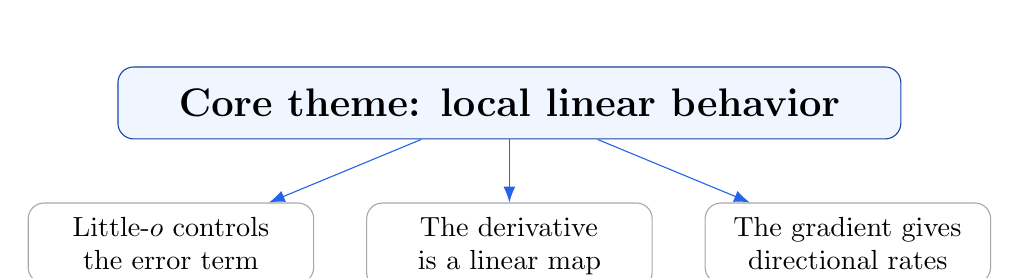
\begin{tikzpicture}[scale=0.82]
\node[draw=accent!70!black,fill=softblue,rounded corners=2mm,minimum width=0.82\textwidth,inner sep=8pt] (A) {\Large\textbf{Core theme: local linear behavior}};
\node[draw=ink!40,fill=white,rounded corners=2mm,below left=8mm and -25mm of A,inner sep=5pt,text width=0.27\textwidth,align=center] (B) {Little-$o$ controls the error term};
\node[draw=ink!40,fill=white,rounded corners=2mm,below=8mm of A,inner sep=5pt,text width=0.27\textwidth,align=center] (C) {The derivative is a linear map};
\node[draw=ink!40,fill=white,rounded corners=2mm,below right=8mm and -25mm of A,inner sep=5pt,text width=0.27\textwidth,align=center] (D) {The gradient gives directional rates};
\draw[-{Latex[length=2mm]},accent] (A) -- (B);
\draw[-{Latex[length=2mm]},accent] (A) -- (C);
\draw[-{Latex[length=2mm]},accent] (A) -- (D);
\end{tikzpicture}%
}
\end{center}

\begin{methodbox}[How these solutions are written]
For each question, the solution first identifies the relevant definition, then translates the problem into that definition, and then carries out the computation.  This is the visible reasoning structure used below: \emph{definition} $\to$ \emph{local formula} $\to$ \emph{limit or derivative computation} $\to$ \emph{final conclusion}.  The diagrams are included only where they clarify the mathematics: little-$o$ scale, linear approximation, differentiability failure at a cusp, gradient direction, and directional derivative level sets.
\end{methodbox}

\newpage
\tableofcontents
\newpage

\section{Problem 1: Little-$o$ notation}

The statement
\[
 f(h)=o(g(h))\quad\text{as }h\to 0
\]
means
\[
 \frac{f(h)}{g(h)}\to 0\quad\text{as }h\to 0,
\]
provided the quotient is interpreted for $h$ sufficiently close to $0$ where $g(h)\neq 0$.  In particular,
\[
 f(h)=o(h)\quad\Longleftrightarrow\quad \frac{f(h)}{h}\to 0.
\]
Equivalently, one may write
\[
 f(h)=h\alpha(h),\qquad \alpha(h)\to 0.
\]
This representation is often the cleanest way to prove algebraic rules for little-$o$ terms.

\begin{center}
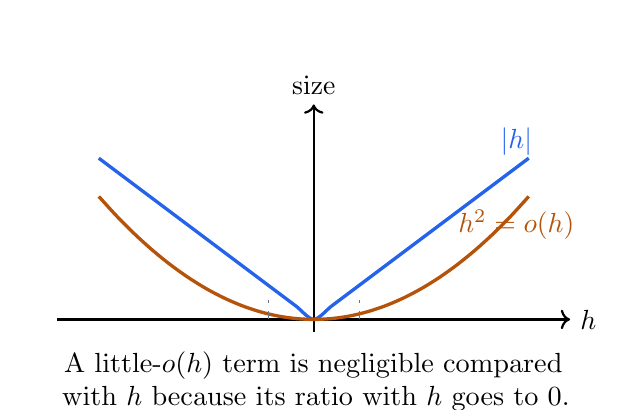
\begin{tikzpicture}[scale=1.05]
\draw[->,thick] (-3.1,0)--(3.1,0) node[right]{$h$};
\draw[->,thick] (0,-0.15)--(0,2.6) node[above]{size};
\draw[domain=-2.6:2.6,smooth,variable=\x,accent,very thick] plot ({\x},{0.75*abs(\x)});
\draw[domain=-2.6:2.6,smooth,variable=\x,accenttwo,very thick] plot ({\x},{0.22*\x*\x});
\node[accent] at (2.45,2.15) {$|h|$};
\node[accenttwo] at (2.45,1.15) {$h^2=o(h)$};
\draw[dashed,muted] (-0.55,0)--(-0.55,0.23);
\draw[dashed,muted] (0.55,0)--(0.55,0.23);
\node[align=center,text width=0.58\textwidth] at (0,-0.75) {A little-$o(h)$ term is negligible compared with $h$ because its ratio with $h$ goes to $0$.};
\end{tikzpicture}
\end{center}

\subsection*{1(i)}
\textbf{Claim.} If $f(h)=o(h)$ and $g(h)=o(h)$, then
\[
 f(h)+g(h)=o(h).
\]

\begin{proof}
By the definition of little-$o$,
\[
 \frac{f(h)}{h}\to 0,\qquad \frac{g(h)}{h}\to 0.
\]
To prove that $f(h)+g(h)=o(h)$, we must prove
\[
 \frac{f(h)+g(h)}{h}\to 0.
\]
Now split the quotient:
\[
 \frac{f(h)+g(h)}{h}=\frac{f(h)}{h}+\frac{g(h)}{h}.
\]
The first term tends to $0$, and the second term also tends to $0$.  Therefore their sum tends to $0+0=0$. Hence
\[
 \frac{f(h)+g(h)}{h}\to 0.
\]
Therefore
\[
 \boxed{f(h)+g(h)=o(h).}
\]
\end{proof}

\subsection*{1(ii)}
\textbf{Claim.} If $f(h)=o(h)$ and $g(h)=o(h)$, then
\[
 f(h)g(h)=o(h^2).
\]

\begin{proof}
By definition,
\[
 \frac{f(h)}{h}\to 0,
 \qquad
 \frac{g(h)}{h}\to 0.
\]
To prove that $f(h)g(h)=o(h^2)$, we must prove
\[
 \frac{f(h)g(h)}{h^2}\to 0.
\]
Rewrite the quotient as a product:
\[
 \frac{f(h)g(h)}{h^2}
 =\left(\frac{f(h)}{h}\right)\left(\frac{g(h)}{h}\right).
\]
Both factors tend to $0$.  Therefore the product tends to $0\cdot 0=0$. Hence
\[
 \frac{f(h)g(h)}{h^2}\to 0.
\]
Therefore
\[
 \boxed{f(h)g(h)=o(h^2).}
\]
\end{proof}

\subsection*{1(iii)}
\textbf{Claim.} If $f(h)=o(h)$ and $g(h)$ is bounded near $0$, then
\[
 f(h)g(h)=o(h).
\]
In particular, if $c$ is a constant, then $cf(h)=o(h)$.

\begin{proof}
Since $g$ is bounded near $0$, there exist constants $M>0$ and $\delta>0$ such that
\[
 |g(h)|\leq M\qquad\text{whenever }0<|h|<\delta.
\]
Since $f(h)=o(h)$,
\[
 \frac{f(h)}{h}\to 0.
\]
Now estimate the quotient that we need:
\[
 \left|\frac{f(h)g(h)}{h}\right|
 = |g(h)|\left|\frac{f(h)}{h}\right|
 \leq M\left|\frac{f(h)}{h}\right|.
\]
The right-hand side tends to $M\cdot 0=0$.  Hence, by the squeeze theorem,
\[
 \frac{f(h)g(h)}{h}\to 0.
\]
Therefore
\[
 \boxed{f(h)g(h)=o(h).}
\]
If $g(h)=c$ is constant, then $g$ is bounded near $0$, so the same result gives
\[
 \boxed{cf(h)=o(h).}
\]
\end{proof}

\newpage
\section{Problem 2: The derivative}

\begin{methodbox}[Definition of differentiability]
Let $F:\R^n\to\R^m$.  The function $F$ is differentiable at $a\in\R^n$ if there exists a linear map
\[
 L:\R^n\to\R^m
\]
such that
\[
 F(a+h)=F(a)+L(h)+o(\norm{h})\quad\text{as }h\to 0.
\]
The linear map $L$ is called the derivative of $F$ at $a$ and is denoted by $\D F(a)$.  Thus the derivative is not just a number; in several variables, it is a linear transformation.
\end{methodbox}

\begin{center}
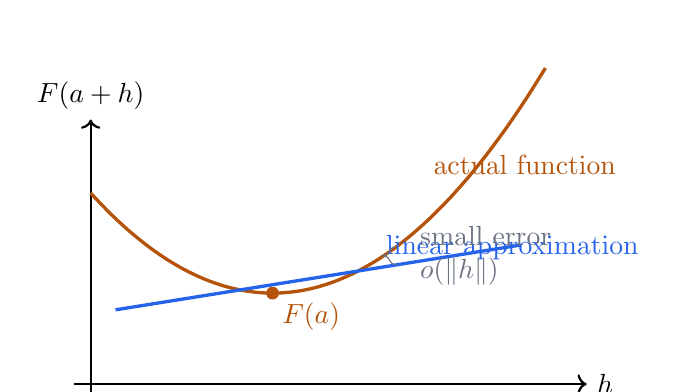
\begin{tikzpicture}[scale=1.05]
\draw[->,thick] (-0.2,0)--(6,0) node[right]{$h$};
\draw[->,thick] (0,-0.2)--(0,3.2) node[above]{$F(a+h)$};
\draw[domain=0:5.5,smooth,variable=\x,accenttwo,very thick] plot ({\x},{0.25*(\x-2.2)^2+1.1});
\draw[domain=0.3:5.2,smooth,variable=\x,accent,very thick] plot ({\x},{0.85+0.16*\x});
\filldraw[accenttwo] (2.2,1.1) circle (2pt) node[below right]{$F(a)$};
\node[accenttwo] at (5.25,2.65) {actual function};
\node[accent] at (5.1,1.65) {linear approximation};
\draw[decorate,decoration={brace,amplitude=5pt},muted] (3.7,1.442)--(3.7,1.663) node[midway,right=5pt,align=left] {small error\\$o(\norm h)$};
\end{tikzpicture}
\end{center}

\subsection*{2(i)(a) Constant map $f(x)=c$}
Suppose $f:\R^n\to\R^m$ is given by $f(x)=c$, where $c\in\R^m$ is fixed.  At any point $a$,
\[
 f(a+h)-f(a)=c-c=0.
\]
Therefore
\[
 f(a+h)=f(a)+0(h)+0.
\]
The linear map is the zero map
\[
 \D f(a)(h)=0.
\]
Hence $f$ is differentiable everywhere and
\[
 \boxed{\D f(a)=0.}
\]

\subsection*{2(i)(b) Affine map $f(t)=(1-t)u+tv$, where $u,v\in\R^3$}
First simplify the expression:
\[
 f(t)=u+t(v-u).
\]
At a point $t_0\in\R$, take an increment $s\in\R$. Then
\[
 f(t_0+s)=u+(t_0+s)(v-u)
 =u+t_0(v-u)+s(v-u).
\]
Since
\[
 f(t_0)=u+t_0(v-u),
\]
we get
\[
 f(t_0+s)=f(t_0)+s(v-u).
\]
There is no error term.  The derivative is the linear map
\[
 \D f(t_0):\R\to\R^3,
 \qquad
 \D f(t_0)(s)=s(v-u).
\]
Therefore
\[
 \boxed{f\text{ is differentiable everywhere and }\D f(t_0)(s)=s(v-u).}
\]

\begin{center}
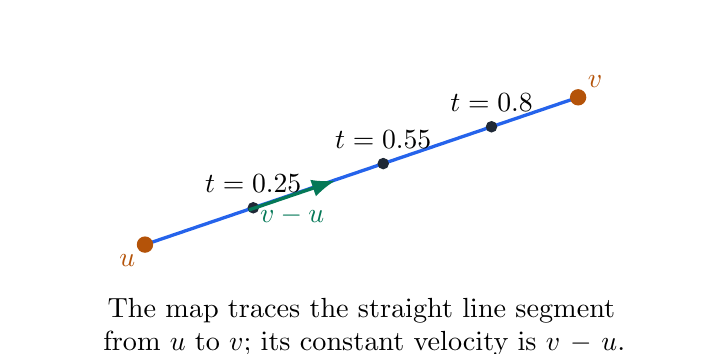
\begin{tikzpicture}[scale=1.1]
\coordinate (U) at (0,0.4);
\coordinate (V) at (5,2.1);
\draw[very thick,accent] (U)--(V);
\filldraw[accenttwo] (U) circle (2.5pt) node[below left]{$u$};
\filldraw[accenttwo] (V) circle (2.5pt) node[above right]{$v$};
\foreach \t/\lab in {0.25/$t=0.25$,0.55/$t=0.55$,0.8/$t=0.8$}
{
\coordinate (P) at ($(U)!\t!(V)$);
\filldraw[ink] (P) circle (1.7pt);
\node[above=2pt] at (P) {\lab};
}
\draw[-{Latex[length=3mm]},deepgreen,very thick] (1.2,0.8)--(2.2,1.14) node[midway,below]{$v-u$};
\node[align=center,text width=0.68\textwidth] at (2.5,-0.55) {The map traces the straight line segment from $u$ to $v$; its constant velocity is $v-u$.};
\end{tikzpicture}
\end{center}

\subsection*{2(i)(c) Linear functional $f(x)=c\cdot x$, where $c\in\R^3$}
Let $a\in\R^3$ and $h\in\R^3$. Then
\[
 f(a+h)=c\cdot(a+h)=c\cdot a+c\cdot h=f(a)+c\cdot h.
\]
Thus the derivative at every point is the same linear functional:
\[
 \D f(a)(h)=c\cdot h.
\]
Therefore
\[
 \boxed{f\text{ is differentiable everywhere and }\D f(a)(h)=c\cdot h.}
\]

\subsection*{2(i)(d) Norm map $f(x)=\norm{x}$}
Assume $f:\R^3\to\R$ is defined by $f(x)=\norm{x}$.

\textbf{Case 1: $a\neq 0$.} We claim that $f$ is differentiable at $a$ and
\[
 \D f(a)(h)=\frac{a\cdot h}{\norm{a}}.
\]
Indeed,
\[
 \norm{a+h}^2=\norm{a}^2+2a\cdot h+\norm{h}^2.
\]
Using the first-order expansion of the square-root function at $\norm a^2>0$,
\[
 \norm{a+h}
 =\norm a+\frac{a\cdot h}{\norm a}+o(\norm h).
\]
Hence
\[
 f(a+h)=f(a)+\frac{a\cdot h}{\norm a}+o(\norm h).
\]
So the derivative is
\[
 \boxed{\D f(a)(h)=\frac{a\cdot h}{\norm a}\quad(a\neq 0).}
\]

\textbf{Case 2: $a=0$.} Suppose, for contradiction, that $f$ is differentiable at $0$. Then there exists a linear map $L:\R^3\to\R$ such that
\[
 \norm{h}=L(h)+o(\norm h).
\]
Take $h=tu$ where $u$ is a fixed unit vector and $t>0$. Then
\[
 t=tL(u)+o(t).
\]
Divide by $t$:
\[
 1=L(u)+o(1),
\]
so $L(u)=1$ for every unit vector $u$. But applying this to $-u$ gives
\[
 L(-u)=1.
\]
Linearity gives $L(-u)=-L(u)=-1$, a contradiction. Therefore $f$ is not differentiable at $0$.

\begin{center}
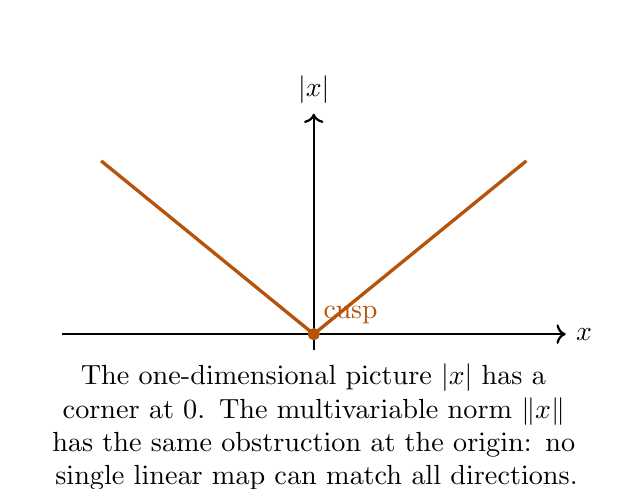
\begin{tikzpicture}[scale=1.0]
\draw[->,thick] (-3.2,0)--(3.2,0) node[right]{$x$};
\draw[->,thick] (0,-0.2)--(0,2.8) node[above]{$|x|$};
\draw[accenttwo,very thick] (-2.7,2.2)--(0,0)--(2.7,2.2);
\filldraw[accenttwo] (0,0) circle (2pt) node[above right]{cusp};
\node[align=center,text width=0.58\textwidth] at (0,-1.18) {The one-dimensional picture $|x|$ has a corner at $0$.  The multivariable norm $\norm{x}$ has the same obstruction at the origin: no single linear map can match all directions.};
\end{tikzpicture}
\end{center}

Thus
\[
 \boxed{\norm{x}\text{ is differentiable exactly at }x\neq 0.}
\]

\subsection*{2(i)(e) Shifted norm map $f(x)=\norm{x-a}$, where $a\in\R^3$}
This is the same norm function shifted by $a$.  Let $x_0$ be the point where we test differentiability.

If $x_0\neq a$, then $x_0-a\neq 0$, and by the previous computation,
\[
 \D f(x_0)(h)=\frac{(x_0-a)\cdot h}{\norm{x_0-a}}.
\]
If $x_0=a$, then
\[
 f(a+h)=\norm{h},
\]
which is not differentiable at $h=0$ by the previous argument. Therefore
\[
 \boxed{f(x)=\norm{x-a}\text{ is differentiable exactly when }x\neq a,}
\]
and at such a point
\[
 \boxed{\D f(x)(h)=\frac{(x-a)\cdot h}{\norm{x-a}}.}
\]

\newpage
\section{Problem 3: Gradient vector}

\begin{methodbox}[Gradient and directional derivative]
For a differentiable scalar field $f:\R^n\to\R$, the gradient is
\[
 \grad f=(f_{x_1},\ldots,f_{x_n}).
\]
For a unit direction $u$, the directional derivative is
\[
 D_u f(x)=\grad f(x)\cdot u.
\]
The maximum rate of change is
\[
 \norm{\grad f(x)},
\]
and it occurs in the direction
\[
 \frac{\grad f(x)}{\norm{\grad f(x)}}
\]
provided $\grad f(x)\neq 0$.
\end{methodbox}

\subsection*{3(i)(a) $f(x,y,z)=x^2-y^2+2z^2$}
Differentiate with respect to each variable separately:
\[
 f_x=2x,
 \qquad
 f_y=-2y,
 \qquad
 f_z=4z.
\]
Therefore
\[
 \boxed{\grad f(x,y,z)=(2x,-2y,4z).}
\]
The question asks for the gradient vector at two different points. Since no points are specified, we choose two illustrative points.

At $P_1=(1,1,1)$,
\[
 \grad f(P_1)=(2,-2,4).
\]
At $P_2=(0,2,-1)$,
\[
 \grad f(P_2)=(0,-4,-4).
\]
Thus
\[
 \boxed{\grad f(1,1,1)=(2,-2,4),\qquad \grad f(0,2,-1)=(0,-4,-4).}
\]

\subsection*{3(i)(b) $f(x,y,z)=x^2y^3z^4$}
Compute each partial derivative:
\[
 f_x=2xy^3z^4,
 \qquad
 f_y=3x^2y^2z^4,
 \qquad
 f_z=4x^2y^3z^3.
\]
Therefore
\[
 \boxed{\grad f(x,y,z)=(2xy^3z^4,\;3x^2y^2z^4,\;4x^2y^3z^3).}
\]
At $P_1=(1,1,1)$,
\[
 \grad f(P_1)=(2,3,4).
\]
At $P_2=(2,1,-1)$,
\[
 \grad f(P_2)=(4,12,-16).
\]
Hence
\[
 \boxed{\grad f(1,1,1)=(2,3,4),\qquad \grad f(2,1,-1)=(4,12,-16).}
\]

\subsection*{3(i)(c) $f(x,y)=e^x\cos y$}
Differentiate:
\[
 f_x=e^x\cos y,
 \qquad
 f_y=-e^x\sin y.
\]
Thus
\[
 \boxed{\grad f(x,y)=(e^x\cos y,-e^x\sin y).}
\]
At $P_1=(0,0)$,
\[
 \grad f(P_1)=(1,0).
\]
At $P_2=(0,\pi/2)$,
\[
 \grad f(P_2)=(0,-1).
\]
Therefore
\[
 \boxed{\grad f(0,0)=(1,0),\qquad \grad f(0,\pi/2)=(0,-1).}
\]

\subsection*{3(ii) $f(x,y,z)=x^2+2y^2-3z^2$ at $(1,1,0)$}
First compute the gradient:
\[
 \grad f(x,y,z)=(2x,4y,-6z).
\]

\subsubsection*{3(ii)(a) Gradient at $(1,1,0)$}
Substitute $(1,1,0)$:
\[
 \grad f(1,1,0)=(2,4,0).
\]
Therefore
\[
 \boxed{\grad f(1,1,0)=(2,4,0).}
\]

\subsubsection*{3(ii)(b) Directional derivative along $(1,-1,2)$}
The vector $(1,-1,2)$ is not a unit vector.  Its length is
\[
 \norm{(1,-1,2)}=\sqrt{1^2+(-1)^2+2^2}=\sqrt6.
\]
So the corresponding unit vector is
\[
 u=\frac{(1,-1,2)}{\sqrt6}.
\]
The directional derivative is
\[
 D_u f(1,1,0)=\grad f(1,1,0)\cdot u.
\]
Therefore
\[
 D_u f(1,1,0)
 =(2,4,0)\cdot\frac{(1,-1,2)}{\sqrt6}
 =\frac{2-4+0}{\sqrt6}
 =-\frac{2}{\sqrt6}.
\]
Thus
\[
 \boxed{D_u f(1,1,0)=-\frac{2}{\sqrt6}=-\frac{\sqrt6}{3}.}
\]

\subsubsection*{3(ii)(c) Direction of maximum rate of change}
The maximum rate of change occurs in the gradient direction.  Since
\[
 \grad f(1,1,0)=(2,4,0),
\]
its length is
\[
 \norm{\grad f(1,1,0)}=\sqrt{2^2+4^2+0^2}=\sqrt{20}=2\sqrt5.
\]
The unit direction of maximum increase is
\[
 \frac{\grad f(1,1,0)}{\norm{\grad f(1,1,0)}}
 =\frac{(2,4,0)}{2\sqrt5}
 =\left(\frac1{\sqrt5},\frac2{\sqrt5},0\right).
\]
Hence
\[
 \boxed{\text{maximum rate}=2\sqrt5,\quad \text{direction}=\left(\frac1{\sqrt5},\frac2{\sqrt5},0\right).}
\]

\subsubsection*{3(ii)(d) Direction of zero rate of change}
A direction $u=(a,b,c)$ gives zero rate of change exactly when
\[
 \grad f(1,1,0)\cdot u=0.
\]
Thus
\[
 (2,4,0)\cdot(a,b,c)=2a+4b=0.
\]
Therefore any unit vector satisfying
\[
 a+2b=0,
 \qquad
 a^2+b^2+c^2=1
\]
gives zero directional derivative.  One simple example is
\[
 u=\frac{(2,-1,0)}{\sqrt5}.
\]
Indeed,
\[
 (2,4,0)\cdot\frac{(2,-1,0)}{\sqrt5}=\frac{4-4}{\sqrt5}=0.
\]
So
\[
 \boxed{\text{yes; for example }u=\frac{(2,-1,0)}{\sqrt5}.}
\]

\begin{center}
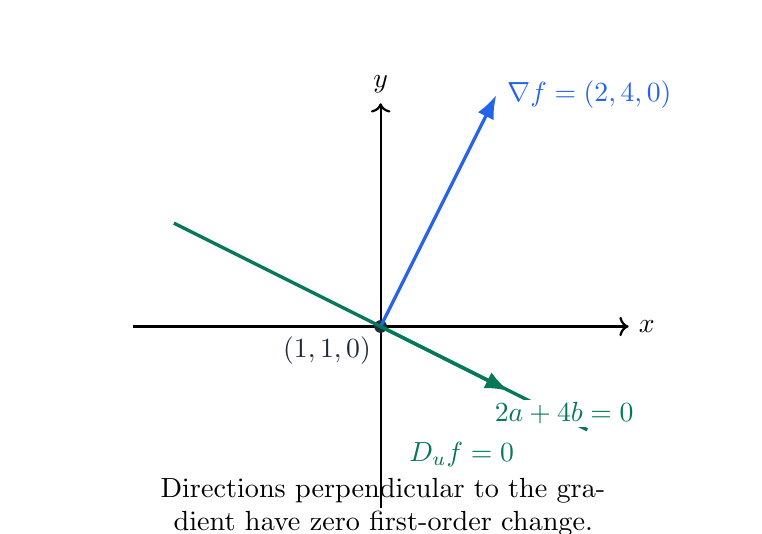
\begin{tikzpicture}[scale=1.05]
\draw[->,thick] (-3,0)--(3,0) node[right]{$x$};
\draw[->,thick] (0,-2.2)--(0,2.7) node[above]{$y$};
\filldraw[ink] (0,0) circle (2pt) node[below left]{$(1,1,0)$};
\draw[-{Latex[length=3mm]},accent,very thick] (0,0)--(1.4,2.8) node[right]{$\grad f=(2,4,0)$};
\draw[deepgreen,very thick] (-2.5,1.25)--(2.5,-1.25);
\node[deepgreen,fill=white,inner sep=1pt] at (2.22,-1.05) {$2a+4b=0$};
\draw[-{Latex[length=3mm]},deepgreen,very thick] (0,0)--(1.55,-0.78);
\node[deepgreen,fill=white,inner sep=1pt] at (0.98,-1.55) {$D_u f=0$};
\node[align=center,text width=0.72\textwidth] at (0,-2.18) {Directions perpendicular to the gradient have zero first-order change.};
\end{tikzpicture}
\end{center}

\subsection*{3(iii) Reconstructing the gradient from directional derivatives}
Let
\[
 \grad f(x)=(A,B).
\]
The problem states that the directional derivative at $x$ along the directions $(2,3)$ and $(1,1)$ are
\[
 \frac1{\sqrt{13}}
 \quad\text{and}\quad
 \sqrt2
\]
respectively.  Since directional derivatives are taken along unit directions, we first normalize the given vectors.

The unit vector in the direction $(2,3)$ is
\[
 \frac{(2,3)}{\sqrt{13}}.
\]
Hence
\[
 D_{(2,3)}f(x)
 = (A,B)\cdot\frac{(2,3)}{\sqrt{13}}
 =\frac{2A+3B}{\sqrt{13}}.
\]
The given value is $1/\sqrt{13}$, so
\[
 \frac{2A+3B}{\sqrt{13}}=\frac1{\sqrt{13}}.
\]
Therefore
\[
 2A+3B=1. \tag{1}
\]

The unit vector in the direction $(1,1)$ is
\[
 \frac{(1,1)}{\sqrt2}.
\]
Hence
\[
 D_{(1,1)}f(x)
 =(A,B)\cdot\frac{(1,1)}{\sqrt2}
 =\frac{A+B}{\sqrt2}.
\]
The given value is $\sqrt2$, so
\[
 \frac{A+B}{\sqrt2}=\sqrt2.
\]
Therefore
\[
 A+B=2. \tag{2}
\]
Solve equations (1) and (2).  From (2),
\[
 A=2-B.
\]
Substitute into (1):
\[
 2(2-B)+3B=1.
\]
So
\[
 4-2B+3B=1,
\]
which gives
\[
 B=-3.
\]
Then
\[
 A=2-(-3)=5.
\]
Thus
\[
 \boxed{\grad f(x)=(5,-3).}
\]

\subsubsection*{3(iii)(b) Directional derivative along $(1,-1)$}
The unit vector in the direction $(1,-1)$ is
\[
 u=\frac{(1,-1)}{\sqrt2}.
\]
Therefore
\[
 D_u f(x)=(5,-3)\cdot\frac{(1,-1)}{\sqrt2}
 =\frac{5+3}{\sqrt2}
 =\frac8{\sqrt2}
 =4\sqrt2.
\]
Hence
\[
 \boxed{D_{(1,-1)}f(x)=4\sqrt2.}
\]

\subsubsection*{3(iii)(c) Sketching the set $\{u:(x;u)=6\}$}
The notation in the question appears to refer to a fixed directional derivative level set.  With the gradient computed above, this means
\[
 \grad f(x)\cdot u=6.
\]
Writing $u=(u_1,u_2)$ gives
\[
 (5,-3)\cdot(u_1,u_2)=6,
\]
so
\[
 5u_1-3u_2=6.
\]
Therefore the set of all direction vectors $u$ satisfying the condition is the straight line
\[
 \boxed{5u_1-3u_2=6.}
\]
If $u$ is required to be a unit direction, then there is no solution, because the largest possible unit-direction derivative is
\[
 \norm{\grad f(x)}=\sqrt{5^2+(-3)^2}=\sqrt{34}<6.
\]
So the line lies outside the unit circle.

\begin{center}
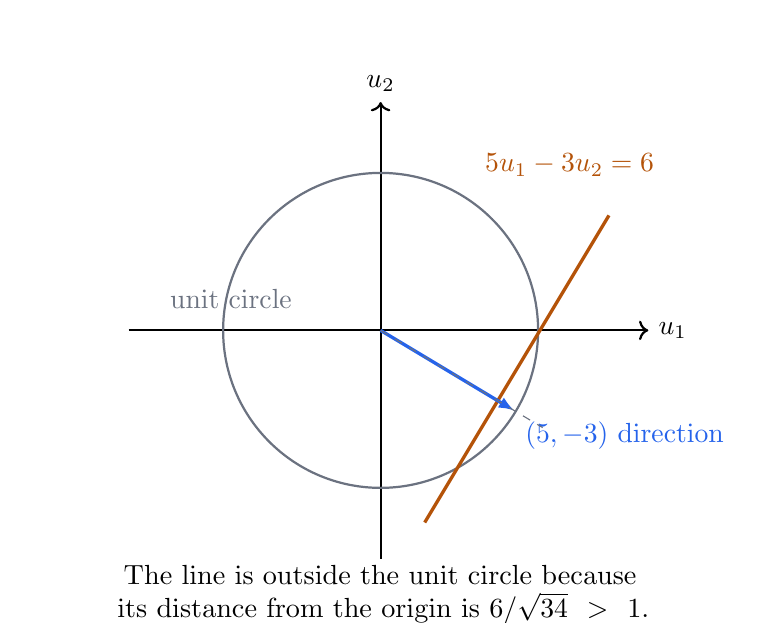
\begin{tikzpicture}[scale=2.0]
\draw[->,thick] (-1.6,0)--(1.7,0) node[right]{$u_1$};
\draw[->,thick] (0,-1.45)--(0,1.45) node[above]{$u_2$};
\draw[muted,thick] (0,0) circle (1);
\node[muted] at (-0.95,0.2) {unit circle};
\draw[accenttwo,very thick] (0.28,-1.22)--(1.45,0.73);
\node[accenttwo,align=center] at (1.2,1.05) {$5u_1-3u_2=6$};
\draw[-{Latex[length=2mm]},accent,very thick] (0,0)--(0.85,-0.51) node[below right]{$(5,-3)$ direction};
\draw[dashed,muted] (0,0)--({30/sqrt(34)/5},{-18/sqrt(34)/5});
\node[align=center,text width=0.72\textwidth] at (0,-1.68) {The line is outside the unit circle because its distance from the origin is $6/\sqrt{34}>1$.};
\end{tikzpicture}
\end{center}

\subsection*{3(iv) Maximum rate of change}

\subsubsection*{3(iv)(a) $f(x,y,z)=\sqrt{x^2+y^2+z^2}$ at $(3,6,-2)$}
This is the norm function, so for $(x,y,z)\neq(0,0,0)$,
\[
 \grad f(x,y,z)=\frac{(x,y,z)}{\sqrt{x^2+y^2+z^2}}.
\]
At $(3,6,-2)$,
\[
 \sqrt{3^2+6^2+(-2)^2}=\sqrt{9+36+4}=\sqrt{49}=7.
\]
Thus
\[
 \grad f(3,6,-2)=\left(\frac37,\frac67,-\frac27\right).
\]
The maximum rate of change is the norm of the gradient:
\[
 \norm{\grad f(3,6,-2)}=1.
\]
It occurs in the direction of the gradient:
\[
 \left(\frac37,\frac67,-\frac27\right).
\]
Therefore
\[
 \boxed{\text{maximum rate}=1,\quad \text{direction}=\left(\frac37,\frac67,-\frac27\right).}
\]

\subsubsection*{3(iv)(b) $f(x,y)=ye^{xy}$ at $(0,2)$}
Compute the gradient:
\[
 f_x=y^2e^{xy},
 \qquad
 f_y=e^{xy}+xye^{xy}=e^{xy}(1+xy).
\]
Thus
\[
 \grad f(x,y)=\left(y^2e^{xy},e^{xy}(1+xy)\right).
\]
At $(0,2)$,
\[
 e^{xy}=e^0=1,
\]
so
\[
 \grad f(0,2)=(4,1).
\]
The maximum rate is
\[
 \norm{(4,1)}=\sqrt{17}.
\]
The direction is
\[
 \frac{(4,1)}{\sqrt{17}}.
\]
Therefore
\[
 \boxed{\text{maximum rate}=\sqrt{17},\quad \text{direction}=\frac{(4,1)}{\sqrt{17}}.}
\]

\subsubsection*{3(iv)(c) $f(x,y)=4y\sqrt{x}$ at $(4,1)$}
The function is defined for $x\geq 0$, and the given point has $x=4>0$, so ordinary partial derivatives apply. Compute
\[
 f_x=4y\cdot\frac1{2\sqrt{x}}=\frac{2y}{\sqrt{x}},
 \qquad
 f_y=4\sqrt{x}.
\]
At $(4,1)$,
\[
 f_x(4,1)=\frac{2}{2}=1,
 \qquad
 f_y(4,1)=4\cdot2=8.
\]
Hence
\[
 \grad f(4,1)=(1,8).
\]
The maximum rate is
\[
 \norm{(1,8)}=\sqrt{1+64}=\sqrt{65}.
\]
The direction is
\[
 \frac{(1,8)}{\sqrt{65}}.
\]
Therefore
\[
 \boxed{\text{maximum rate}=\sqrt{65},\quad \text{direction}=\frac{(1,8)}{\sqrt{65}}.}
\]

\begin{center}
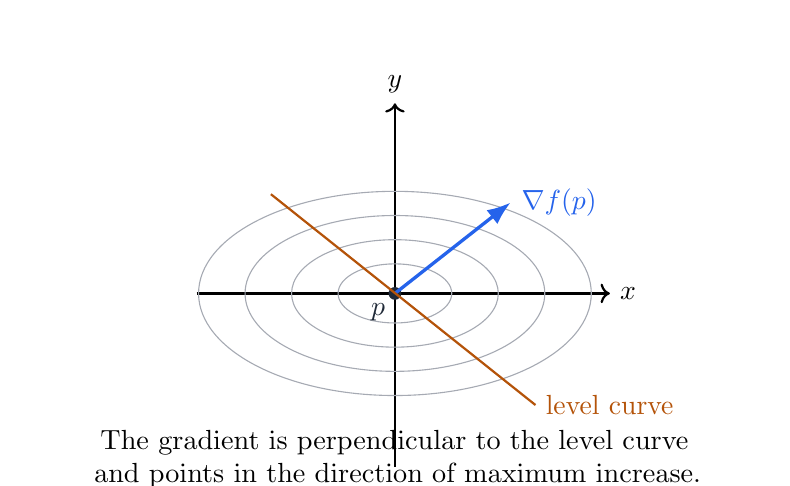
\begin{tikzpicture}[scale=1.05]
\draw[->,thick] (-2.4,0)--(2.6,0) node[right]{$x$};
\draw[->,thick] (0,-2.1)--(0,2.3) node[above]{$y$};
\foreach \r in {0.55,1.0,1.45,1.9}
{\draw[muted!60] (0,0) ellipse ({1.25*\r} and {0.65*\r});}
\filldraw[ink] (0,0) circle (2pt) node[below left]{$p$};
\draw[-{Latex[length=3mm]},accent,very thick] (0,0)--(1.4,1.1) node[right]{$\grad f(p)$};
\draw[accenttwo,thick] (-1.5,1.2)--(1.7,-1.35) node[right]{level curve};
\node[align=center,text width=0.75\textwidth] at (0,-2.0) {The gradient is perpendicular to the level curve and points in the direction of maximum increase.};
\end{tikzpicture}
\end{center}

\newpage
\subsection*{3(v) Properties of the gradient}

\begin{warningbox}[Correction of printed identities]
The printed problem appears to contain typographical errors in the scalar multiple and product rules.  The correct standard identities are
\[
 \grad(\lambda f)=\lambda\grad f,
 \qquad
 \grad(fg)=f\grad g+g\grad f.
\]
The quotient rule printed in the problem is the standard quotient rule.
\end{warningbox}

Assume $f,g$ are differentiable scalar-valued functions on a suitable open domain in $\R^n$, and $\lambda$ is a constant.

\subsubsection*{3(v)(i) $\grad f=0$ iff $f$ is constant}
If $f$ is constant, then every partial derivative is zero, so
\[
 \grad f=0.
\]
Conversely, suppose $\grad f=0$ everywhere on $\R^n$.  Take any two points $a,b\in\R^n$.  Define the one-variable function
\[
 \phi(t)=f(a+t(b-a)),\qquad 0\leq t\leq 1.
\]
By the chain rule,
\[
 \phi'(t)=\grad f(a+t(b-a))\cdot(b-a).
\]
Since $\grad f=0$ everywhere,
\[
 \phi'(t)=0.
\]
Therefore $\phi$ is constant on $[0,1]$, so
\[
 \phi(0)=\phi(1).
\]
That is,
\[
 f(a)=f(b).
\]
Since $a,b$ were arbitrary, $f$ is constant. Hence
\[
 \boxed{\grad f=0\text{ iff }f\text{ is constant on }\R^n.}
\]
On a general disconnected domain, the conclusion is true on each connected component.

\subsubsection*{3(v)(ii) Sum and difference rule}
For each coordinate $x_i$,
\[
 \frac{\partial}{\partial x_i}(f\pm g)
 =\frac{\partial f}{\partial x_i}\pm\frac{\partial g}{\partial x_i}.
\]
Therefore, assembling the partial derivatives into a vector,
\[
 \boxed{\grad(f\pm g)=\grad f\pm\grad g.}
\]

\subsubsection*{3(v)(iii) Scalar multiple rule}
For each coordinate $x_i$,
\[
 \frac{\partial}{\partial x_i}(\lambda f)
 =\lambda\frac{\partial f}{\partial x_i}.
\]
Therefore
\[
 \boxed{\grad(\lambda f)=\lambda\grad f.}
\]

\subsubsection*{3(v)(iv) Product rule}
For each coordinate $x_i$,
\[
 \frac{\partial}{\partial x_i}(fg)
 =f\frac{\partial g}{\partial x_i}+g\frac{\partial f}{\partial x_i}.
\]
Therefore
\[
 \boxed{\grad(fg)=f\grad g+g\grad f.}
\]

\subsubsection*{3(v)(v) Quotient rule}
At points where $g\neq 0$,
\[
 \frac{f}{g}=f\cdot g^{-1}.
\]
Using the product rule and the chain rule,
\[
 \grad\left(\frac{f}{g}\right)
 =\grad(fg^{-1})
 =f\grad(g^{-1})+g^{-1}\grad f.
\]
Since
\[
 \grad(g^{-1})=-g^{-2}\grad g,
\]
we get
\[
 \grad\left(\frac{f}{g}\right)
 =-\frac{f}{g^2}\grad g+\frac1g\grad f.
\]
Putting the terms over the same denominator,
\[
 \grad\left(\frac{f}{g}\right)
 =\frac{g\grad f-f\grad g}{g^2}.
\]
Therefore
\[
 \boxed{\grad\left(\frac{f}{g}\right)=\frac{g\grad f-f\grad g}{g^2},\qquad g\neq 0.}
\]

\newpage
\section*{Final answer summary}
\addcontentsline{toc}{section}{Final answer summary}

\begin{answerbox}[Compact checklist]
\begin{enumerate}[label=\textbf{\arabic*.},leftmargin=2em]
\item Little-$o$ rules follow directly by dividing by the comparison scale and using limit laws.
\item Constant maps have zero derivative; affine maps have constant derivative; linear maps are their own derivative; $\norm{x}$ is differentiable away from $0$ but not at $0$; $\norm{x-a}$ is differentiable away from $a$ but not at $a$.
\item Gradients computed:
\[
\grad(x^2-y^2+2z^2)=(2x,-2y,4z),
\]
\[
\grad(x^2y^3z^4)=(2xy^3z^4,3x^2y^2z^4,4x^2y^3z^3),
\]
\[
\grad(e^x\cos y)=(e^x\cos y,-e^x\sin y).
\]
\item For $f=x^2+2y^2-3z^2$ at $(1,1,0)$:
\[
\grad f=(2,4,0),\quad D_{(1,-1,2)}f=-\frac2{\sqrt6},\quad \max=2\sqrt5.
\]
\item From the two given directional derivatives in Problem 3(iii):
\[
\grad f(x)=(5,-3),\quad D_{(1,-1)}f(x)=4\sqrt2.
\]
\item Maximum-rate answers:
\[
\sqrt{x^2+y^2+z^2}\text{ at }(3,6,-2):\quad \max=1,
\]
\[
 ye^{xy}\text{ at }(0,2):\quad \max=\sqrt{17},
\]
\[
4y\sqrt{x}\text{ at }(4,1):\quad \max=\sqrt{65}.
\]
\item Gradient rules are the componentwise derivative rules: linearity, product rule, and quotient rule.
\end{enumerate}
\end{answerbox}

\end{document}
